\documentclass[brazil,12pt,plain]{article}
\usepackage[utf8]{inputenc}
\usepackage[T1]{fontenc}
\usepackage[brazil]{babel}
\usepackage{graphicx}
\usepackage{subfig}
\usepackage[a4paper,top=1cm,bottom=1cm,left=1cm,right=1cm]{geometry}

\newcommand{\code}[1]{\texttt{#1}}

\begin{document}

\section{Definições}
\label{sec:definicoes}

\begin{figure}[!h]
  \centering
  \subfloat[Melodia]{
    \includegraphics[scale=1]{5a-sinfonia}
  }
  \subfloat[Contorno]{
    \includegraphics[scale=1]{c-3120}
  }
  \caption{Fragmento da 5ª Sinfonia de Beethoven}
\end{figure}

\section{Representações de contornos}
\label{sec:repr-de-cont}

\begin{figure}[!h]
  \centering
  \includegraphics[scale=1]{ly-2031}    
  \caption{Melodias de contorno (2 0 3 1)}
  \label{fig:melodias}
\end{figure}

\begin{enumerate}
\item Representação simbólica
  \begin{itemize}
  \item Contorno: Z(2 0 3 1)
  \item Elementos: Z$_0=2$, Z$_1=0$, Z$_2=3$ e Z$_3=1$
  \end{itemize}
\item Representação gráfica
  \begin{figure}[!h]
    \centering
    \includegraphics[scale=1]{c-2031}
    \caption{Representação gráfica}
    \label{fig:representacao-grafica}
  \end{figure}
\end{enumerate}

\section{Representação de operações}
\label{sec:repr-de-oper}

\begin{itemize}
\item Retrógrado de X(1 2 3): $retr(X(1\;2\;3))=Y(3\;2\;1)$
\item Transposição de X(1 2 3) com fator 2: $transp(X(1\;2\;3)\;2)=W(3\;4\;5)$
\item Concatenação de operações: $transp(retr(inv(rot(X(1\;2\;3))\;2))\;3)$
\end{itemize}

\section{Operações implementadas}
\label{sec:oper-impl}

\begin{enumerate}
\item Retrogradação
\item Inversão
\item Transposição
\item Rotação
\item Expansão de intervalos
\item Classe de contornos
\item Série de contornos adjacentes
\item Vetor de séries de contornos
\item Vetores I e II de classes de contorno
\item Matriz de comparação
\end{enumerate}

\section{O Goiaba}
\label{sec:o-goiaba}

\subsection{Representação}
\label{sec:representacao}

\begin{itemize}
\item Contornos simples: \code{(5 9 6)}
\item Contornos com duração: \code{((0 5)(1 9)(2 6))}
\end{itemize}

\subsection{Classes e macros}
\label{sec:classes-e-macros}

\begin{itemize}
\item \texttt{ponto}: \code{(x y)}\\
  \code{\#p(x y)}
\item \texttt{contorno-simples}: \code{(y w)}\\
  \code{\#s(y w)}
\item \texttt{contorno-duracao}: \code{((x y) (z
    w))}\\
  \code{\#d(\#p(x y) \#p(x y))}
\end{itemize}

\begin{verbatim}
(defmethod transpor ((objeto contorno-duracao) fator)
  (map-contorno-duracao #L(transpor !1 fator) (pontos objeto)))

(defmethod transpor ((objeto contorno-simples) fator)
  (map-contorno-simples #L(+ !1 fator) (pontos objeto)))
\end{verbatim}

\subsection{Saída do Goiaba}
\label{sec:saida-do-goiaba}

\begin{verbatim}
(let ((contorno #s(0 5 3 4 1 3)))
  (simple-plot
   contorno "original" :blue
   (transpor contorno 2) "transposição" :green
   (retrogradar contorno) "retrógrado" :red
   (inverter contorno) "inversão" :orange
   (rotacionar contorno 1) "rotação" :darkcyan
   ))
\end{verbatim}

  \begin{figure}[!h]
    \centering
    \subfloat[Dois contornos]{
      \includegraphics[scale=1]{expansao}
    }

    \subfloat[Vários contornos]{
      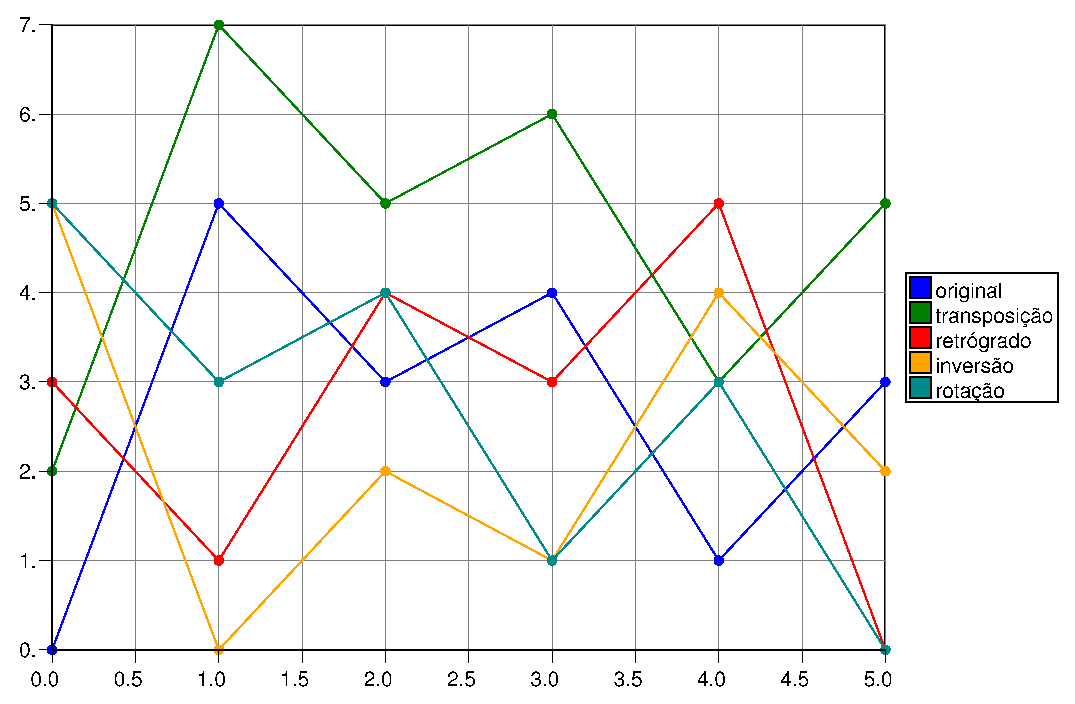
\includegraphics[scale=1]{contornos}
    }
    \caption{Saída do Goiaba}
  \end{figure}

\end{document}

